A crucial matter when designing a controller for automated operation of robotic surgery tools is the necessity of guaranteed patient safety. The system has to not only be able to prevent the surgery tool from entering certain regions, e.g. penetrating the wall of the heart or cutting an artery, but to guarantee that this cannot happen under any circumstances.


Casting the controller design problem as an optimization problem with constraints, such as \gls{mpc}, could in principle guarantee that the tool would not enter a predefined area. Indeed, \gls{mpc} is a method which is very popular at the higher abstraction layers, such as setpoint control \citep{bib:mpc_simon} which is the case in this specific study. However, most solvers such as the Matlab plugin \texttt{cvx} requires convexity in the performance function and its constraints to be able to find a global minimum. This will at best be a lucky special case that unsafe regions can be defined through a convex function.  
Furthermore, \gls{mpc} is mostly used in systems with slow dynamics, i.e. dynamics where the time constant is measured in seconds or even minutes \citep{bib:mpc_slow}. This is obviously due to heavy online computations and numerous iterations. Systems containing these time constants are usually thermal systems and not mechanical systems. Additionally, the feasibility of the optimization problem is not very transparent and it is well known that \texttt{cvx} is very likely to crash due to infeasibility.
%, but a hard constraint would fail to follow the dynamics of a moving area boundary such as a beating heart. 

Another very elegant and computationally efficient approach to the safe controller analysis and design problem is the use of barrier certificates, which provide a formal proof of safe operation in infinite time horizon \citep{bib:prajna_framework,bib:safety}. This chapter describes the requirements for the construction of barrier certificates along with notation used in relation to these.
%


%dealing with those topics within robotic surgeries feature necessary conditions to guarantee the patient safety and to avert patient trauma .



\section{Constraints for a Barrier Certificate}\label{sec:safety-def}

When a barrier certificate can be found for a (closed-loop) dynamical system, the controller is guaranteed to be safe. In the following the notion of safety is defined in order to describe the guarantee extent of a barrier certificate. A general state-space representation of an $n$-dimensional non-linear system is considered:
\begin{equation}
\dot{x} = f_{cl}(x) + h(x)\,d = f(x) + g(x)\,u + h(x)\,d
\label{eq:general_statespace}
\end{equation}
\begin{tabular}{rl} 
where &  \\
\gls{x} &  is the state, $x(t) \in \mathbb{R}^n$\\
\gls{u} & is the control input, $u(t) \in \mathbb{R}^m$\\
\gls{d} & is the disturbance input, $d(t) \in D \subseteq \mathbb{R}^p$ \\
\gls{f} & is a non-linear function, $f:\mathbb{R}^n \rightarrow \mathbb{R}^n$\\
\gls{g} & is a non-linear function, $g:\mathbb{R}^n \rightarrow \mathbb{R}^{n \times m}$\\
\gls{h} & is a non-linear function, $h:\mathbb{R}^n \rightarrow \mathbb{R}^{n \times p}$
\end{tabular}\\

Consider a subspace of the state-space $\mathcal{X}\subseteq\mathbb{R}^n$ defining e.g. the physically feasible states for the system in \autoref{eq:general_statespace}. Within this region $\mathcal{X}$, define the two non-intersecting subspaces $\mathcal{X}_u\subset\mathcal{X}$ and $\mathcal{X}_0\subseteq\mathcal{X}$, defining an unsafe  and a safe region, respectively. The unsafe region contains the states which the trajectory of the system must never enter, e.g. for a surgical robot this space could be the collection of veins and organs near the operation site, for which perforation is prohibited. The safe region contains all the states which the trajectory of the system is allowed to and may be required to enter, e.g. the operation site and a region for entering the area in the abdomen.
Now safety of a closed-loop control system is given according to \citep{bib:safety,bib:prajna_framework} as:
%\begin{exa}

\begin{defn}[Safety of a System]\label{def:safety}
Denote a trajectory starting in $x(0)=x_0$ and with bounded disturbance function $\bar{d}:\mathbb{R}_{\geq 0}\rightarrow D$ by $\phi_{x_0}^{\bar{d}}$, defined by 
\begin{equation}
\frac{d \phi_{x_0}^{\bar{d}} }{dt} = f_{cl}\left( \phi_{x_0}^{\bar{d}} (t) \right) + h\left( \phi_{x_0}^{\bar{d}} (t) \right) \bar{d}(t)
\end{equation}
The system $\Gamma_{cl} = (f_{cl},h,\mathcal{X},\mathcal{X}_0,\mathcal{X}_u,D)$ is unsafe if there exists a $t \in [0,$\gls{T}$]$ such that the trajectory $\phi_{\mathcal{X}_0}^{\bar{d}}:\,[0,T]\rightarrow \mathbb{R}^n$ with initial state $x_0\in \mathcal{X}_0$ and bounded disturbance function $\bar{d}$ satisfies
\begin{flalign}
\left( \phi_{\mathcal{X}_0}^{\bar{d}}([0,t]) \cap \mathcal{X}_u \right) \neq \emptyset \kk \text{and} \kk 
\phi_{\mathcal{X}_0}^{\bar{d}}([0,t]) \subseteq \mathcal{X}
\label{eq:defsafety}
\end{flalign}
\noindent
The system $\Gamma_{cl}$ is safe if there are no unsafe trajectories.
\end{defn}

%\vspace{-0.2cm}
%
%\begin{longtable}{p{.9\textwidth} p{.1\textwidth} p{.1\textwidth}} 
%Where  & & \\
%\gls{fcl} is a potential non-linear function with the closed loop characteristic:\\ \kk $f_\text{cl}: x \mapsto f(x)+g(x)k(x)$ where \gls{k} is the feedback gain with the map $k: \mathbb{R}^n \rightarrow \mathbb{R}^m$ & [$\cdot$] &  \\
%\gls{X} is the set of all allowed states & [$\cdot$] &  \\
%\gls{X0} is the set of all allowed initial states & [$\cdot$] &  \\
%\gls{Xu} is the set of all unsafe states & [$\cdot$] &  \\
%\gls{phi} is the set of all allowed initial conditions with the bounded disturbance input \gls{dbar} & [$\cdot$]
%\end{longtable}

A graphical interpretation of \autoref{eq:defsafety} is shown in \autoref{fig:defsafety}.

\begin{figure}[H]
	\center
	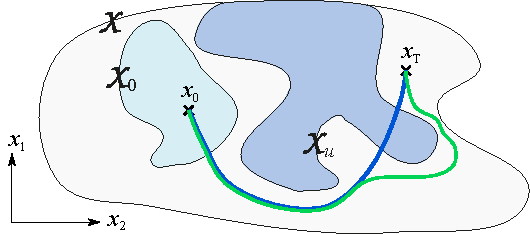
\includegraphics[width=0.6\textwidth]{safety.pdf}	
	\caption{Graphical interpretation of \autoref{eq:defsafety} in the state space. The blue trajectory is unsafe because $\left( \phi_{\mathcal{X}_0}^{\bar{d}}([0,t]) \cap \mathcal{X}_u \right) \neq \emptyset$, while the green trajectory is safe.}
	\label{fig:defsafety}
\end{figure}
%\end{exa}

Disturbances are not considered in the scope of this project, and hence $d\in D$ is considered to be zero in the remainder of this thesis.

For the system in \autoref{eq:general_statespace} safety can be guaranteed if a barrier certificate for the system exists. A barrier certificate is defined as a function of the system state, satisfying a set of inequalities, entailing that its zero level set in the state space forms a barrier between the safe set of initial states $\mathcal{X}_0$ and the unsafe set $\mathcal{X}_u$, thereby certifying system safety \citep{bib:prajna_framework}.


If a barrier certificate can be defined, safety can be guaranteed for the closed-loop system in the region $\mathcal{X}$, with unsafe region $\mathcal{X}_u$, defined by positive values of the barrier function, and (safe) initial region $\mathcal{X}_0$, defined by non-positive values of the barrier function. In the below the notation $L_{f_{cl}}B(x)$ denotes the Lie derivative of \gls{bar} along the vector field of the closed-loop system $f_{cl}(x)$, corresponding to the time derivative of the barrier function i.e.
\begin{equation}
L_{f_{cl}}B(x)=\frac{dB(x)}{dx}f_{cl}(x)=\frac{dB(x)}{dx}\frac{dx(t)}{dt}=\frac{dB(x(t))}{dt}
\end{equation}

Requiring that the time derivative of the barrier function must be nonpositive on the entire set $\mathcal{X}$ (see \autoref{def:barrier_certificate}) corresponds to the value of the barrier function decreasing over time, hence seeking the minimum of the (convex) barrier certificate. Requiring the trajectory of the state to start within the safe set $\mathcal{X}_0$ this means that the trajectory will never cross the zero level set and enter the unsafe set $\mathcal{X}_u$, as this set only contains values of the barrier function larger than the initial value.

\begin{defn}[Barrier Certificate]\label{def:barrier_certificate}	
If a barrier certificate can be constructed as a continuous and differentiable function $B(x):\mathcal{X} \rightarrow \mathbb{R}$ adhering to the following inequalities  \citep{bib:prajna_framework}:
\begin{subequations}\label{eq:barrier_constraints}
\begin{flalign}
B(x) &\leq 0 \kk  \forall \hspace{2mm} x \in \mathcal{X}_0  \label{cer1}\\
B(x) &> 0  \kk  \forall \hspace{2mm} x \in \mathcal{X}_u \label{cer2} \\
L_{f_{cl}}B(x) &\leq 0 \kk  \forall \hspace{2mm} x \in \mathcal{X} \label{cer3}
\end{flalign}
\end{subequations}
Then safety of the closed-loop system $f_{cl}(x)$, as defined in \autoref{def:safety}, is guaranteed. 
\end{defn}


From \autoref{eq:barrier_constraints} it can be seen that the function $B(x)$ must be constructed such that its zero level set delimits and separates the safe and the unsafe regions, while the Lie derivative constraint imposes that the derivative $dB(x)/dx$ must have the opposite sign of the state derivative $dx/dt$ for any state within the region $\mathcal{X}$ where $B(x)$ is defined. 
Note how according to \autoref{cer3} the barrier certificate requires mere stability and not asymptotic stability ($L_{f_{cl}}B(x)<0$) of the system trajectory. This is rarely enough when dealing with physical systems, however, mathematically it is sufficient.

Furthermore from \autoref{cer3} it is deduced that a controller incorporating the barrier certificate in its design will ensure stability if $B(x)$ has a finite minimum value. This entails that $B(x) $ is radially unbounded if $\mathcal{X}$ encompasses the entire state-space:
\begin{equation}
\underset{x\rightarrow \pm\infty}{\lim} B(x)= \infty \kk \text{if} \kk \mathcal{X}=\mathbb{R}^n
\end{equation}

\subsubsection{Nexus to Lyapunov Functions}
\vspace*{-3mm}
As it can be seen from \autoref{eq:barrier_constraints} the definition of a barrier certificate strongly resembles that of a Lyapunov function, and indeed the Lie derivative nonpositivity constraint is identical to the time derivative constraint to a Lyapunov function $V(x)$, a Lyapunov candidate function for a stable system given by
\vspace*{-5mm}
%\begin{equation}
%\dot{x}  = f(x) = \frac{d x}{d t} \qquad
%\left\{ \begin{array}{r l l}
%L_fB(x) \hspace*{-2mm}&= \tfrac{d B(x)}{d x} f(x) \hspace*{-2mm}&= \tfrac{d B(x)}{d x} \frac{d x}{d t}\\
%\dot{V}(x) \hspace*{-2mm}&= \tfrac{d V(x)}{d t} \hspace*{-2mm}&= \tfrac{d V(x)}{d x}\tfrac{d x}{d t}
%\end{array} \right. \label{eq:dBdt_dVdt}
%\end{equation}
\begin{subequations}\label{eq:lyap}
\begin{align}
V(x) &> 0 \kk \forall x \in \mathbb{R}\setminus\{0\}\\
\dot{V}(x) &\leq 0 \label{eq:lyap_stable}
\end{align}	
and for a system with an asymptotically stable equilibrium in $x=0$, \autoref{eq:lyap_stable} is replaced by
\vspace*{-2mm}
\begin{equation}
\dot{V}(x) < 0 \kk \forall x \in \mathbb{R}\setminus\{0\}
\end{equation}
\end{subequations}
As such a barrier certificate can be seen as an offset Lyapunov function with negative values in the safe region. The stable focus may also be offset from $x=0$. However, a barrier function may also take other (non-convex) forms. 



\subsection{Approaches to the Problem}
Two approaches to the problem of designing/verifying safety controllers through barrer certificates are used in the following. In \autoref{part:cbf} barrier certificates are constructed by hand, and guaranteed safe controllers are designed according to the method given in \citep{bib:org_control}, which is described in \autoref{chap:cbf}. The safe controller is used in combination with a linear state space controller designed through pole placement for setpoint control in the safe region. In \autoref{chap:cbf_1d_static} and \ref{chap:cbf_1d_dynamic} system models of different orders are considered in 1D space, with static and dynamic boundaries (zero level sets) of the barrier function, respectively, while in \autoref{chap:cbf_3d_static} and \ref{chap:cbf_3d_dynamic} systems models are considered in 3D space. \textcolor{red}{Correct this when the chapters are written!}

In \autoref{part:putinar} similar linear state-space controllers are designed for setpoint control and their safety is then validated by the construction of a barrier certificate using Putinar's Positivstellensatz according to \citep{bib:sos_putinar_lasserre}, as described in \autoref{chap:putinar}. Similarly to \autoref{part:cbf} the following chapters verify controller safety for system models of different orders in 1D and 3D space, with static and dynamic boundaries (zero level sets) of the barrier function.
%\autoref{chap:sos_1d_static} \autoref{chap:sos_1d_dynamic} \autoref{chap:sos_3d_static} \autoref{chap:sos_3d_dynamic}



%The design of a safe controller features the property that a supplied control signal ensures compliance of the definition described in \autoref{sec:safety-def}.







